Mathematicians are often skeptical of proofs relying on extensive computation.
A landmark example is the \emph{four-color theorem}, which states that any planar graph can be colored with at most four colors.
In 1879, Alfred Kempe published a proof attempt that was discovered to be incorrect 11 years later by Headwood~\cite{Walters2004ItAT,Wilson2002GraphsCA}.
% \footnote{The main idea of Kempe's proof was salvaged by Headwood to prove the weaker \emph{five-color theorem}, and it is still a building block in the theory of planar colorings~\cite{Walters2004ItAT}.}
A full proof was not found until 1976, when Kenneth Appel and Wolfgang Haken used a computer to check the 1\,834 cases that might contain a counterexample~\cite{appelFourColorProblem1978}.
Their proof was controversial, and small errors were indeed found in their initial calculations~\cite{Walters2004ItAT,Wilson2002GraphsCA}.
In 2005, Georges Gonthier formalized a full proof of the four-color theorem in the \textsf{Coq} proof assistant~\cite{gonthierFourColourTheorem2008a}, thus laying to rest any lingering doubts about the correctness of the result.
% To this day, all proofs known for this theorem require the assistance of computers.

The four-color theorem is far from the end of the story when it comes to computer-assisted mathematics.
An emerging trend is to use SAT solvers (or other automated reasoning tools) to prove mathematical theorems by analyzing finite objects~\cite{avigad2023mathematics}.
To name a few examples,
Keller's conjecture~\cite{brakensiek2023resolution},
the packing chromatic number of the infinite grid~\cite{Subercaseaux_Heule_2023},
the Pythagorean triples problem~\cite{Heule_2016},
Lam's problem~\cite{21bright_sat_based_resolution_lams_problem},
and one case of the Erd\H{o}s discrepancy conjecture~\cite{konev2014sat}
were all resolved or confirmed using SAT solvers.
All such SAT-based results follow a common structure. To show that a mathematical theorem $\mathcal{T}$ holds, one proves the following:

\begin{enumerate}
  \item (\textbf{Reduction Theorem}) There is a finite object $\mathcal{O}$ such that either (\emph{positive case}) if $\mathcal{O}$ exists then $\mathcal{T}$ holds, or (\emph{negative case}) if $\mathcal{O}$ does not exist then $\mathcal{T}$ holds. %\footnote{Note that $\mathcal{T}$ can be a statement concerning infinite objects, as for example in the case of Keller's conjecture~\cite{brakensiek2023resolution}.}
  \item (\textbf{Encoding Theorem}) There is a CNF formula $\varphi_{\mathcal{O}}$ such that either (\emph{positive case}) if $\varphi_{\mathcal{O}}$ is satisfiable then $\mathcal{O}$ exists, or (\emph{negative case}) if $\varphi_{\mathcal{O}}$ is unsatisfiable then $\mathcal{O}$ does not exist.
  \item (\textbf{SAT Result}) In the \emph{positive case}, a SAT solver finds a satisfying assignment for $\varphi_{\mathcal{O}}$, and in the \emph{negative case}, a SAT solver finds that $\varphi_{\mathcal{O}}$ is unsatisfiable.
\end{enumerate}

% Unfortunately, the formula $\varphi_{\mathcal{O}}$ concerning the existence of $\mathcal{O}$ is often too large or computationally hard to be solved directly, so a fourth step is added to the above method: a \textbf{Re-encoding Theorem} showing that $\varphi_{\mathcal{O}}$ is equisatisfiable with a simpler formula $\phi_{\mathcal{O}}$.
% All the examples we mentioned above add this step, and so will we.
% Furthermore,
% One of the benefits of using a SAT solver for mathematical proofs is that in the \emph{positive case}, it is usually possible to construct the desired object $\mathcal{O}$ from a satisfying assignment to $\phi_{\mathcal{O}}$, and then by exhibiting $\mathcal{O}$, the correctness of theorem $\mathcal{T}$ can be easily verified by humans.
It is worth noting that the \emph{negative case} of SAT-based mathematical proofs presents a particular challenge for human trust: the unsatisfiability proofs emitted by SAT solvers are usually too large for human verification, and depend crucially on the correctness of the encoding.\footnote{In the positive case, the correctness of the encoding is not even required, as an incorrect encoding might still lead to obtaining a concrete object $\mathcal{O}$ that satisfies the desired properties, proving the intended theorem regardless.}
% \todo[inline]{CC: I don't like how this paragraph is structured. The negative case isn't inherently \emph{harder}. Instead, the method of verifying the overall result is different: rather than constructing an actual object we can see or compute on, we have to rely on a non-existence result. Thus, the reduction must be correct, as errors can't be caught the same way they can be in a physical construction.\\ BS: I disagree; the NP vs coNP asymmetry is exactly about how easy it is to convince a verifier of existence vs. non-existence results.}
In particular, the proof by Heule and Scheucher for the \emph{Empty Hexagon Number} uses 180 terabytes in the \textsf{LRAT} format, and around 80 terabytes in the \textsf{DRAT} format~\cite{emptyHexagonNumber}. Most of the other SAT-based proofs mentioned above result in even larger proofs~\cite{Heule_2016,lambTwohundredterabyteMathsProof2016,heule2017schur,Subercaseaux_Heule_2023}.
% For example, the resolution of the Boolean Pythagorean triples problem required an unsatisfiability proof of 200 terabytes~\cite{Heule_2016,lambTwohundredterabyteMathsProof2016}, and the proof of Schur's number five required 2 petabytes~\cite{heule2017schur}.
This raises a fundamental question for computational mathematics:
\begin{center}
  \emph{How can we enhance trust for a theorem $\mathcal{T}$ that relies on a very long unsatisfiability proof?}
\end{center}

% \begin{figure}[ht]
    \centering
    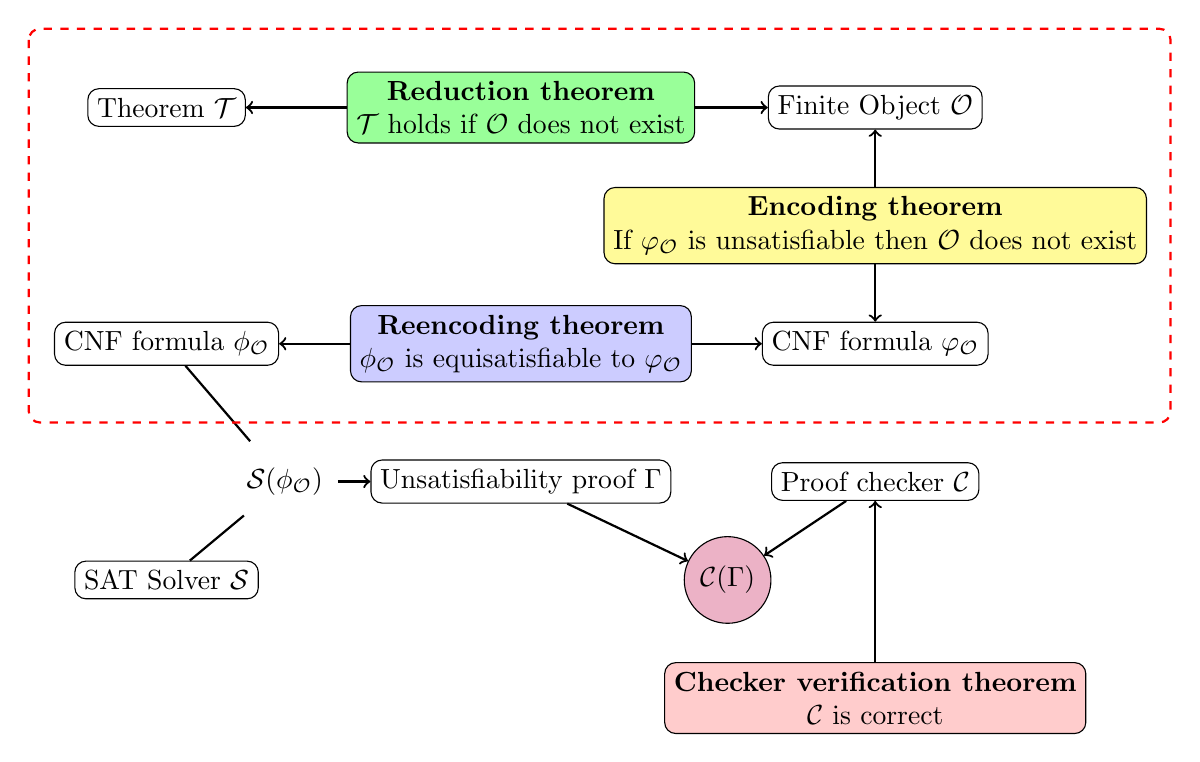
\begin{tikzpicture}
      \node[draw, rounded corners] (theorem) at (0,0) {Theorem $\mathcal{T}$};
      \node[draw, rounded corners] (object) at (9,0) { Finite Object $\mathcal{O}$};
      \node[draw, rounded corners, align=center, fill=green!40!white] (tiffo) at (4.5,0) { \textbf{Reduction theorem}\\$\mathcal{T}$ holds if $\mathcal{O}$ does not exist};
      \draw[->, thick] (tiffo) -- (theorem);
      \draw[->, thick] (tiffo) -- (object);
      \node[draw, rounded corners, align=center] (varphi) at (9, -3) {CNF formula $\varphi_{\mathcal{O}}$};
      \node[draw, rounded corners, align=center, fill=yellow!40!white] (encoding) at (9, -1.5) { \textbf{Encoding theorem}\\If $\varphi_{\mathcal{O}}$ is unsatisfiable then $\mathcal{O}$ does not exist};
      \draw[->, thick] (encoding) -- (object);
      \draw[->, thick] (encoding) -- (varphi);
      \node[draw, rounded corners] (phi) at (0, -3) {CNF formula $\phi_{\mathcal{O}}$};
      \node[draw, rounded corners, align=center, fill=blue!20!white] (equisat) at (4.5, -3) { \textbf{Reencoding theorem}\\$\phi_{\mathcal{O}}$ is equisatisfiable to $\varphi_{\mathcal{O}}$};
      \draw[->, thick] (equisat) -- (phi);
      \draw[->, thick] (equisat) -- (varphi);
      \node[draw, rounded corners] (solver) at (0, -6) {SAT Solver $\mathcal{S}$};
      \node[draw, rounded corners] (unsat-proof) at (4.5, -4.75) {Unsatisfiability proof $\Gamma$};
      \node[circle] (solverphi) at (1.5, -4.75) {$\mathcal{S}(\phi_{\mathcal{O}})$};
      \draw[-, thick] (solver) -- (solverphi);
      \draw[-, thick] (phi) -- (solverphi);
      \draw[->, thick] (solverphi) -- (unsat-proof);
      \node[draw, rounded corners] (checker) at (9, -4.75) {Proof checker $\mathcal{C}$};
      \node[circle, draw, fill=purple!30!white] (checkerphi) at (7.125, -6) {$\mathcal{C}(\Gamma)$};
      \draw[->, thick] (unsat-proof) -- (checkerphi);
      \draw[->, thick] (checker) -- (checkerphi);
      \node[draw, rounded corners, align=center, fill=red!20!white] (checkerCorrectness) at (9, -7.5) { \textbf{Checker verification theorem}\\$\mathcal{C}$ is correct};
  
      \draw[->, thick] (checkerCorrectness) -- (checker);
      \draw[red, dashed, thick, rounded corners] (-1.75,1) -- (-1.75, -4) -- (12.75, -4) -- (12.75, 1) -- cycle;
    \end{tikzpicture}
    \caption{General structure of the verification pipeline for a SAT-based theorem in the \emph{negative case}. The dashed rectangle encloses the main focus of this paper, whereas for the rest of the proof we leverage already existing tools.}\label{fig:proof-structure}
  \end{figure}

The main contribution of this article is to provide a formally-verified proof of such a theorem in Lean, thus tackling several aspects of the question above in the particular context of discrete geometry.
% the context of discrete geometry, addressing different aspects of the question above.
% Our proof pipeline involves several components, as illustrated in~\Cref{fig:proof-structure} and described in the rest of the paper.
All our code is publicly available at \url{https://github.com/bsubercaseaux/EmptyHexagonLean}.
% \footnote{CC: I'm not sure this characterization is correct. For example, another group of researchers verified in Coq the encoding used in the Pythagorean Triples problem, thus verifying that result. One could say that our contribution is the first \emph{end-to-end} verification, but I don't see how it's inherently distinct from what this other group did with the Pythagorean Triples problem.}
% BS: Thanks Cayden, you were right.

\subparagraph*{The Empty Hexagon Number.}
In the 1930s,
following a suggestion of Esther Klein,
Erd\H{o}s and Szekeres showed that for any $k \geq 3$,
one can find a sufficiently large number $n$
such that every $n$ points in \emph{general position}
(i.e., with no three points collinear)
contain a convex \emph{$k$-gon}, i.e., a convex polygon with $k$ vertices~\cite{35erdos_combinatorial_problem_geometry}.
The minimal such $n$ is denoted $g(k)$.
The same authors later showed that $g(k) > 2^{k-2}$
and conjectured that this bound is tight~\cite{60erdos_some_extremum_problems_elementary_geometry}.
Indeed, it is known that $g(5) = 9$ and $g(6) = 17$,
with the latter result obtained by Szekeres and Peters 71 years after the initial conjecture
via exhaustive computer search~\cite{06szekeres_computer_solution_17_point_erdos_szekeres_problem}.
Larger cases remain open,
with $g(k) \leq 2^{k+o(k)}$ the best known upper bound~\cite{suk2017erdos,holmsen2017two}.
This problem is now known as the \emph{Happy End Problem}
as it led to the marriage of Klein and Szekeres.

In a similar spirit,
Erd\H{o}s defined $h(k)$
to be the minimal number of points in general position
that is guaranteed to contain a \emph{$k$-hole},
or \emph{empty $k$-gon},
meaning a convex $k$-gon with no other point inside.
It is easy to check that $h(3) = 3$ and $h(4) = 5$.
In 1978, Harborth established that $h(5) = 10$~\cite{Harborth1978}.
Surprisingly, for $k \geq 7$ a point set with no $k$-hole
can always be constructed
as demonstrated by Horton in 1983~\cite{hortonSetsNoEmpty1983}.
The only case left open was thus $h(6)$.
The \emph{Empty Hexagon Theorem},
establishing $h(6)$ to be finite,
was proven independently by Gerken and Nicolás in 2006~\cite{gerkenEmptyConvexHexagons2008,nicolasEmptyHexagonTheorem2007}.
As of last year,
the known range of values for $h(6)$ was quite large,
at $30 \leq h(6) \leq 1717$
as refined by Valtr in 2008~\cite{valtr},
until a breakthrough by Heule and Scheucher~\cite{emptyHexagonNumber}.
These authors used a SAT solver
to prove that $h(6) \leq 30$,
a result we refer to as the \emph{Empty Hexagon Number}.
Now that all the values of $h$ are known,
and especially given the extensive computation involved in its proofs,
we propose that the final chapter in the story
should be a formal verification of the Empty Hexagon Number.

\subparagraph*{Verification of SAT proofs.}
Formal verification plays a crucial rule in the SAT community,
for example in verified solvers~\cite{10maric_formal_verification_modern_sat_solver_shallow_embedding_isabelle_hol,oeVersatVerifiedModern2012,skotam_creusat_2022}
and proof checking~\cite{lammichEfficientVerifiedSAT2020,tanVerifiedPropagationRedundancy2023}.
Despite this,
not many mathematical proofs obtained through SAT-solving
have been formally verified.

In SAT-based combinatorial geometry,
formal verification was pioneered by Marić~\cite{19maric_fast_formal_proof_erdos_szekeres_conjecture_convex_polygons_most_six_points}
who improved on the speed needed to obtain $g(6) = 17$,
and trustworthiness of this result,
by replacing bespoke code with a SAT encoding
and verifying this encoding in \textsf{Isabelle/HOL}.
We give a detailed comparison between this work and ours in~\Cref{sec:related-work}.
The solution to the Pythagorean triples problem
was verified in the \textsf{Coq} proof assistant
by Cruz-Filipe and coauthors~\cite{formalPythagoreanTriples,LPAR-21:Formally_Proving_Boolean_Pythagorean}.
Giljeg\r{a}rd and Wennerbreck~\cite{GilAndWennerbeck} provide a \textsf{CakeML} library
for verified SAT encodings
which they demonstrated on different puzzles
(e.g., Sudoku, Kakuro, the \emph{N-queens} problem).
As far as verifying SAT encodings in Lean,
we base our work on that of Codel, Avigad, and Heule~\cite{Cayden}.

\subparagraph*{Lean.} Kickstarted by Leonardo de Moura in 2013~\cite{demouraLeanTheoremProver2015}, the Lean theorem prover has arguably become the most popular for formalizing modern breakthroughs in mathematical research.
On the one hand, the recent success of projects such as the~\emph{Liquid Tensor Experiment}~\cite{Castelvecchi2021}, or the proof of~the polynomial Freiman–Ruzsa conjecture~\cite{gowers2023conjecture, slomanATeamMathProves2023} has brought significant attention to~Lean. % as an interactive theorem prover.
On the the other hand, the \textsf{mathlib} project~\cite{The_mathlib_Community_2020} has already cemented the foundations of many areas of mathematics, thus allowing modern results to be formalized much more easily by relying on hundreds of thousands of existing lines of code. In this spirit, we connect our formalization to~\textsf{mathlib} as much as possible.

\subparagraph*{Outline of the paper.}
\Cref{sec:geometry} discusses the basic geometric aspects of the problem.  Then,~\Cref{sec:triple-orientations} is devoted to \emph{triple orientations}, a fundamental tool in computational geometry to discretely represent problems involving an a priori continuous space (i.e., $\mathbb{R}^2$).
 Triple orientations are the basis of Heule and Scheucher's SAT encoding.
 Next,~\Cref{sec:properties-of-sigma} proves properties of orientations that reduce the search space,
and correspond to~\Cref{eq:constraint-4,eq:constraint-5}.
% Then,~\Cref{sec:empty-triangle} presents how the previous elements are already enough to formalize a SAT-based proof for the \emph{Empty Triangle Theorem}, a much simpler problem involving only triangles.
The Empty Hexagon Number requires a sophisticated encoding, presented in~\Cref{fig:full-encoding}, for which two main ingredients are required. First,~\Cref{sec:symmetry-breaking} deals with symmetry breaking, proving that one can assume, without loss of generality, that points are in \emph{canonical position}, a definition that includes points being simultaneously sorted from left-to-right and by angle with respect to the leftmost point.
%  Namely, that one can assume without loss of generality the following two properties at the same time: (i) points are labeled from left to right without two of them having the same $x$-coordinate, and (ii) the triples $(p_1, p_i, p_j)$ are always oriented counterclockwise for $i < j$.
Then,~\Cref{sec:empty-hexagon-number} deals with the efficient re-encoding of Heule and Scheucher, the crucial piece to make the proof of $h(6) = 30$ feasible. Next,~\Cref{sec:leansat} presents the preliminary \textsf{LeanSAT} library, which is used to create a SAT encoding that is provably connected to the geometric properties it describes. We compare our work with its closest precedent due to Marić~\cite{19maric_fast_formal_proof_erdos_szekeres_conjecture_convex_polygons_most_six_points} in~\Cref{sec:related-work}. We conclude in~\Cref{sec:conclusions} by discussing next steps towards the formal verification of other Erd\H{o}s-Szekeres-type problems.

\begin{figure}
  \caption{Encoding based on that of Heule and Scheucher for the Empty Hexagon Number~\cite{emptyHexagonNumber}. Unsatisfiability of the formula below for $n=30$ implies $h(6) \leq 30$, as detailed throughout the paper. }
  \label{fig:full-encoding}
% \begin{framed}
  \begin{spreadlines}{16pt}
\begin{gather}
\hfsetfillcolor{green!10}
\hfsetbordercolor{green!60!black}
\tikzmarkin{b}(4.25,-0.9)(-0.5,0.5)
  \cvar_{i; a,b, c} \rightarrow \left(\left(\orvar_{a,b,c} \leftrightarrow \orvar_{a, i, c}  \right) \land \left(\orvar_{a,b,c} \leftrightarrow \ov{\orvar_{a, i, b}}  \right)\right) \text{ for all } 2 \leq a < i < b < c \leq n\label{eq:constraint-1}\\
  \cvar_{i; a,b, c} \rightarrow \left(\left(\orvar_{a,b,c} \leftrightarrow \orvar_{a, i, c}  \right) \land \left(\orvar_{a,b,c} \leftrightarrow \ov{\orvar_{b, i, c}}  \right)\right) \text{ for all } 2 \leq a < b < i < c \leq n\label{eq:constraint-2}\\
  \bigwedge_{\substack{a < i < c\\ i \neq b}} \ov{\cvar_{i; a,b,c}} \rightarrow \hvar_{a, b, c} \quad \text{ for all } 2 \leq a < b < c \leq n\label{eq:constraint-3}
  \tikzmarkend{b}\\
\tikzmarkin{a}(3.5,-0.3)(-0.5,0.5)
\left(\orvar_{a, b, c} \land \orvar_{a, c, d}\right) \rightarrow \orvar_{a, b, d} \text{ for all } 2 \leq a < b < c < d \leq n\label{eq:constraint-4}\\
\left(\ov{\orvar_{a, b, c}} \land \ov{\orvar_{a, c, d}}\right) \rightarrow \ov{\orvar_{a, b, d}} \text{ for all } 2 \leq a < b < c < d \leq n \tikzmarkend{a}\label{eq:constraint-5}\\
\hfsetfillcolor{blue!10}
\hfsetbordercolor{blue!60!black}
\tikzmarkin{c}(0.45,-0.4)(-0.5,0.5)
    % \orvar_{1, b, c} \quad \text{ for all } 2 \leq b < c \leq n \label{eq:constraint-6}\\
    \left(\orvar_{\lceil \frac{n}{2} \rceil -1, \lceil \frac{n}{2} \rceil,\lceil \frac{n}{2} \rceil+1}, \ldots, \orvar_{2,3,4} \right) \succeq_{\text{lex}} \left(\orvar_{\lfloor \frac{n}{2}\rfloor +1,  \lfloor \frac{n}{2}\rfloor +2, \lfloor \frac{n}{2}\rfloor +3}, \ldots, \orvar_{n-2, n-1, n} \right)\tikzmarkend{c}\label{eq:constraint-6}\\
\hfsetfillcolor{orange!10}
\hfsetbordercolor{orange!60!black}
\tikzmarkin{d}(3.235,-0.3)(-0.5,0.5)
  \left(\ov{\orvar_{a,b,c}} \land \ov{\orvar_{b,c,d}}\right) \rightarrow \uvar_{a, c, d} \quad \text{ for all } 2 \leq a < b < c < d \leq n\label{eq:constraint-7}\\
  \left(\uvar_{a,b,c} \land \ov{\orvar_{b,c,d}} \land \hvar_{a,b,d}\right)\rightarrow \ufvar_{a, c, d} \quad \text{ for all } 2 \leq a < b < c < d \leq n,\; a+1<b\label{eq:constraint-8}\\
  \left(\orvar_{a, b, c} \land \orvar_{b, c, d}\right) \rightarrow \vvar_{a, c, d} \quad \text{ for all } 2 \leq a < b < c < d \leq n \tikzmarkend{d}\label{eq:constraint-9}\\
\hfsetfillcolor{red!10}
\hfsetbordercolor{red!60!black}
\tikzmarkin{e}(3.6,-0.5)(-0.5,0.5)
  \ov{\ufvar_{a,d,e}} \lor \ov{\orvar_{a, b, e}} \quad \text { for all } 2 \leq a < d < e \leq n, \; a < b < e\label{eq:constraint-10}\\
  \ov{\ufvar_{a,d,e}} \lor \orvar_{d, e, f} \quad \text { for all } 2 \leq a < d < e < f\leq n\label{eq:constraint-11}\\
  \ov{\uvar_{a,c,d}} \lor \ov{\vvar_{a, c', d}} \lor \ov{\hvar_{a,c,c'}} \quad \text{ for all } 2 \leq a < c < c' < d \leq n\label{eq:constraint-12}\\
  \ov{\uvar_{a,c,d}} \lor \ov{\vvar_{a, c', d}} \lor \ov{\hvar_{a,c',c}} \quad \text{ for all } 2 \leq a < c' < c < d \leq n\label{eq:constraint-13}\\
  \ov{\vvar_{a,c,d}} \lor \ov{\orvar_{c, d, e}} \lor \ov{\hvar_{a,c,e}} \quad \text{ for all } 2 \leq a < c < d < e \leq n\label{eq:constraint-14x}
\tikzmarkend{e}
  \end{gather}
\end{spreadlines}
% \end{framed}
\end{figure}

